\def\JClientAone{0.5}
\def\JManagerAone{0.75}
\def\JClientAtwo{0.5}
\def\JManagerAtwo{1}
\def\JClientBone{1}
\def\JManagerBone{0.5}
\def\JClientBtwo{1}
\def\JManagerBtwo{0.25}
\def\JClientCone{0.75}
\def\JManagerCone{0.5}
\def\JClientCtwo{0.75}
\def\JManagerCtwo{1}
\def\InitialDeterministic{42}
\def\RevisedDeterministic{42}
\def\CostDeterministic{0.0}
\def\CostLabelDeterministic{0.0000}
\def\InitialSingle{30}
\def\RevisedSingle{42}
\def\CostSingle{2.131419}
\def\CostLabelSingle{2.1314}
\def\InitialMulti{22}
\def\RevisedMulti{42}
\def\CostMulti{5.6347994}
\def\CostLabelMulti{5.6348}
\def\CostRatio{2.64}

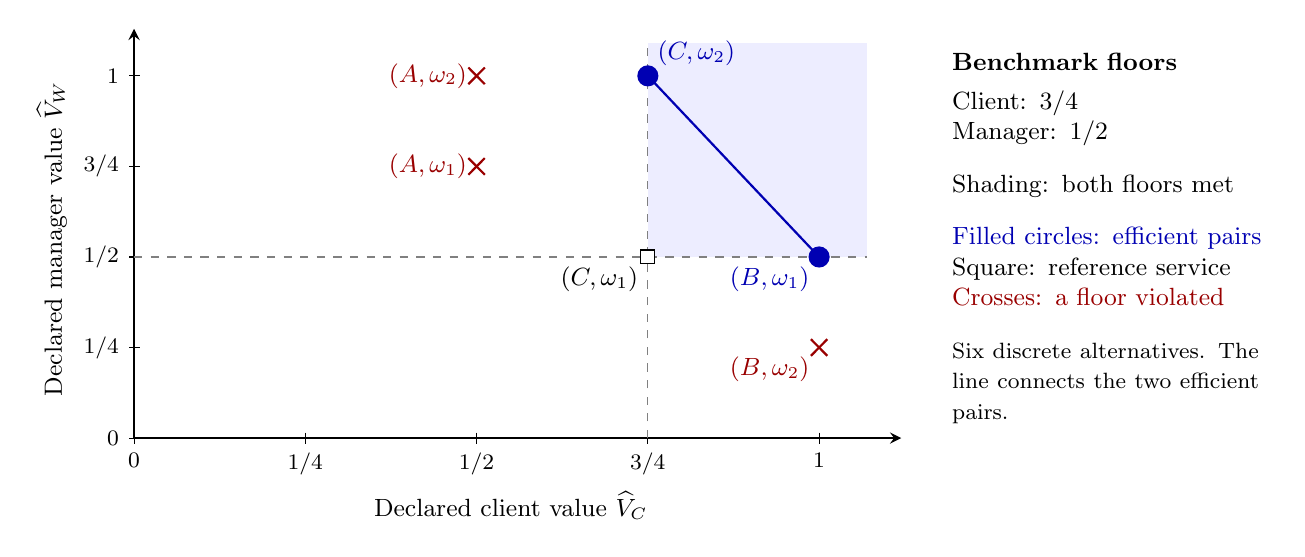
\begin{tikzpicture}[x=8.7cm,y=4.6cm,font=\small,>=stealth]
  \fill[blue!7] (\JClientCone,\JManagerCone) rectangle (1.07,1.09);
  \draw[->,thick] (0,0) -- (1.12,0);
  \draw[->,thick] (0,0) -- (0,1.13);
  \foreach \v/\lab in {0/0,0.25/{1/4},0.5/{1/2},0.75/{3/4},1/1} {
    \draw (\v,0.015) -- (\v,-0.015) node[below,font=\footnotesize] {$\lab$};
    \draw (0.008,\v) -- (-0.008,\v) node[left,font=\footnotesize] {$\lab$};
  }
  \node[below] at (0.55,-0.12) {Declared client value $\widehat V_C$};
  \node[rotate=90] at (-0.12,0.55) {Declared manager value $\widehat V_W$};
  \draw[dashed,gray] (\JClientCone,0) -- (\JClientCone,1.09);
  \draw[dashed,gray] (0,\JManagerCone) -- (1.07,\JManagerCone);
  \draw[thick,blue!70!black] (\JClientCtwo,\JManagerCtwo) -- (\JClientBone,\JManagerBone);
  \node[circle,fill=blue!70!black,inner sep=2.7pt] at (\JClientCtwo,\JManagerCtwo) {};
  \node[above right,text=blue!70!black] at (\JClientCtwo,\JManagerCtwo) {$(C,\omega_2)$};
  \node[circle,fill=blue!70!black,inner sep=2.7pt] at (\JClientBone,\JManagerBone) {};
  \node[below left,text=blue!70!black] at (\JClientBone,\JManagerBone) {$(B,\omega_1)$};
  \node[rectangle,draw,fill=white,inner sep=2.5pt] at (\JClientCone,\JManagerCone) {};
  \node[below left] at (\JClientCone,\JManagerCone) {$(C,\omega_1)$};
  \foreach \x/\y in {\JClientAone/\JManagerAone,\JClientAtwo/\JManagerAtwo,\JClientBtwo/\JManagerBtwo} {
    \draw[thick,red!60!black] (\x-0.012,\y-0.023) -- (\x+0.012,\y+0.023);
    \draw[thick,red!60!black] (\x-0.012,\y+0.023) -- (\x+0.012,\y-0.023);
  }
  \node[left,text=red!60!black] at (\JClientAone,\JManagerAone) {$(A,\omega_1)$};
  \node[left,text=red!60!black] at (\JClientAtwo,\JManagerAtwo) {$(A,\omega_2)$};
  \node[below left,text=red!60!black] at (\JClientBtwo,\JManagerBtwo) {$(B,\omega_2)$};
  \node[anchor=north west,align=left,text width=4.0cm] at (1.18,1.09)
    {\textbf{Benchmark floors}\\[3pt]
     Client: $3/4$\\Manager: $1/2$\\[8pt]
     Shading: both floors met\\[8pt]
     \textcolor{blue!70!black}{Filled circles: efficient pairs}\\
     Square: reference service\\
     \textcolor{red!60!black}{Crosses: a floor violated}\\[8pt]
     {\footnotesize Six discrete alternatives. The line connects the two efficient pairs.}};
\end{tikzpicture}
